
		\subsubsection{Error analysis}
			When there is many potential realizations for a single LTI filter,
			we can see that the choice of one realization among the others is very related to the error analysis in output.
			Considering a filter $\mathcal{H}$ and it's SIF, following the algorithm \ref{sifalgo}, in finite precision, we get the following equations:

			\begin{eqnarray} \label{sifalgoerr}
				\boldsymbol{t}^*(k+1) = - \boldsymbol{J'}\boldsymbol{t}^*(k+1) + \boldsymbol{M} \boldsymbol{x}^*(k) + \boldsymbol{N} \boldsymbol{u}(k) + \boldsymbol{\varepsilon_t}(k)\\
				\boldsymbol{x}^*(k+1) = \boldsymbol{K}\boldsymbol{t}^*(k+1) + \boldsymbol{P} \boldsymbol{x}^*(k) + \boldsymbol{Q_i} \boldsymbol{u}(k) + \boldsymbol{\varepsilon_x}(k) \\
				\boldsymbol{y}^*(k+1) = \boldsymbol{L}\boldsymbol{t}^*(k+1) + \boldsymbol{R} \boldsymbol{x}^*(k) + \boldsymbol{S_i} \boldsymbol{u}(k) + \boldsymbol{\varepsilon_y}(k) 
			\end{eqnarray}

			Where $\boldsymbol{\varepsilon_z}$ is the error vector at instant k, and $\boldsymbol{z}^*(k)$ the computed vector (supposed with no error), with $\boldsymbol{z} \in {\boldsymbol{t},\boldsymbol{x},\boldsymbol{y}}$.

			Let's denote $\varepsilon(k)$ the error vector at instant k:
			\begin{equation} \label{epsilonmatrix}
			\boldsymbol{\varepsilon}(k)=
						\begin{pmatrix}
							\boldsymbol{\varepsilon_t}(k) \\
							\boldsymbol{\varepsilon_x}(k) \\
							\boldsymbol{\varepsilon_y}(k) 
						\end{pmatrix}
			\end{equation}

			We denote $\boldsymbol{\delta t}(k+1)=\boldsymbol{z}_i^*(k)-\boldsymbol{z}_i(k)$ the error at instant k,
			considering computations errors and loopback, for $\boldsymbol{z} \in {\boldsymbol{t},\boldsymbol{x},\boldsymbol{y}}$.
			We get then:
			\begin{eqnarray} \label{deltaerr}
				\boldsymbol{\delta t}^*(k+1) = - \boldsymbol{J'}\boldsymbol{\delta t}^*(k+1) + \boldsymbol{M} \boldsymbol{\delta x}^*(k) + \boldsymbol{\varepsilon_t}(k)\\
				\boldsymbol{\delta x}^*(k+1) = \boldsymbol{K}\boldsymbol{\delta t}^*(k+1) + \boldsymbol{P} \boldsymbol{\delta x}^*(k) + \boldsymbol{\varepsilon_x}(k) \\
				\boldsymbol{\delta y}^*(k+1) = \boldsymbol{L}\boldsymbol{\delta t}^*(k+1) + \boldsymbol{R} \boldsymbol{\delta x}^*(k) + \boldsymbol{\varepsilon_y}(k) 
			\end{eqnarray}

			This new algorithm corresponds here to the algorithm of the SIF of a filter $\mathcal{H}_{\boldsymbol{\varepsilon}}$,
			which describes the behaviour of computation errors at time k on the output.
			The linearity condition allows to decompose the real $\mathcal{H}^*$ filter in two distinct filters:
			\begin{itemize}
				\item $\mathcal{H}$ the absolute filter in infinite precision
				\item $\mathcal{H}_{\boldsymbol{\varepsilon}}$ the error filter
			\end{itemize}

			\begin{figure}[h] 
			  \centering
			  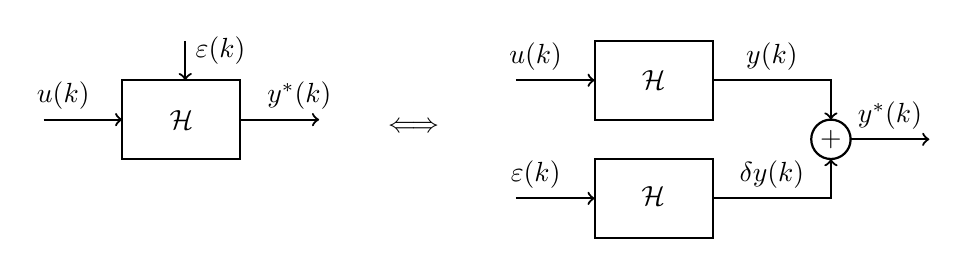
\begin{tikzpicture}[x=1cm,y=1cm]
				\draw (-9, 0.5) -- (-8,0.5) [->, thick] node[above,near start]{$\boldsymbol{u}(k)$};
				\draw (-7.2, 1.5) -- (-7.2,1.0) [->, thick] node[right,near start]{$\boldsymbol{\varepsilon}(k)$};
				\draw (-6.5, 0.5) -- (-5.5,0.5) [->, thick] node[above,near end]{$\boldsymbol{y}^*(k)$};
				\draw (-8,0.0) rectangle ++(1.5,1)[thick] node [midway]{$\mathcal{H}$}; 
				\draw (-2,0.5) rectangle ++(1.5,1)[thick] node [midway]{$\mathcal{H}$}; 
				\draw (-3, 1) -- (-2,1) [->, thick] node [above,near start]{$\boldsymbol{u}(k)$}; 
				\draw (-0.5, 1)  -- (1,1) -- (1,0.5) [->, thick] node[xshift=-0.75cm,yshift=0.8cm]{$\boldsymbol{y}(k)$}; 

				\draw (-2,-1) rectangle ++(1.5,1)[thick] node [midway]{$\mathcal{H}_{\abserr}$}; 
				\draw (-3, -0.5) -- (-2,-0.5) [->, thick] node[above,near start]{$\boldsymbol{\varepsilon}(k)$};
				\draw (-0.5, -0.5) -- (1,-0.5) -- (1,0) [->, thick] node [xshift=-0.75cm,yshift=-0.2cm]{$\boldsymbol{\delta y}(k)$}; 

				\draw (1,0.25) circle (0.25) [thick] node {$+$}; 
				\draw (1.25,0.25) -- (2.25,0.25)[->, thick] node [above,midway] {$\boldsymbol{y}^*(k)$};

				\node (arrow) at (-4.3,0.4) {$\iff$};
			  \end{tikzpicture}

			\caption{A signal view of the error propagation with respect to the ideal filter \label{fig:ltierror}}
			\end{figure}


		According to \ref{zmatrix}, we have:

		\begin{equation} \label{zepsmatrix}
		\boldsymbol{Z_\varepsilon}=
					\begin{pmatrix}
						\boldsymbol{-J} & \boldsymbol{M} & \boldsymbol{M}_t \\
						\boldsymbol{K} & \boldsymbol{P} & \boldsymbol{M}_x \\
						\boldsymbol{L} & \boldsymbol{R} & \boldsymbol{M}_y 
					\end{pmatrix}
		\end{equation}

		with:
		\begin{eqnarray} \label{deltaerr}
			\boldsymbol{M}_t=(\boldsymbol{I}_{n_t} \boldsymbol{0}_{n_t \times n_x} \boldsymbol{0}_{n_t \times n_y}), \\
			\boldsymbol{M}_x=(\boldsymbol{0}_{n_x \times n_x} \boldsymbol{I}_{n_x} \boldsymbol{0}_{n_x \times n_y}), \\
			\boldsymbol{M}_y=(\boldsymbol{0}_{n_y \times n_t} \boldsymbol{0}_{n_y \times n_x} \boldsymbol{I}_{n_y}),
		\end{eqnarray}

		$\mathcal{H}_{\boldsymbol{\varepsilon}}$ is a filter with ($n_t+n_x+n_u$) inputs and $n_y$ outputs.
		\begin{proposition}
			The transfert function of filter $\mathcal{H_{\boldsymbol{\varepsilon}}}$, denoted $\boldsymbol{H}_\varepsilon$, is defined as follows:
			\begin{equation}
				\boldsymbol{H}_{\varepsilon}: \rightarrow \boldsymbol{C_Z}(z\boldsymbol{I}_n-\boldsymbol{A_Z})^{-1}\boldsymbol{M}_1 +\boldsymbol{M}_2 \hspace{5pt} \forall z \in \mathbb{C}
			\end{equation}
			with $\boldsymbol{A_Z}$ and $\boldsymbol{C_Z}$ the matrices defined by \ref{abcdtranspose} and
			\begin{equation}
				\boldsymbol{M_1}=(\boldsymbol{KJ}^{-1}   \hspace{10pt}\boldsymbol{I}_{n_x} \hspace{10pt} \boldsymbol{0}), 
				\boldsymbol{M_2}=(\boldsymbol{LJ}^{-1}  \hspace{10pt}\boldsymbol{0} \hspace{10pt}\boldsymbol{I}_{n_y}), 
			\end{equation}
		\end{proposition}
